\documentclass{article}

\usepackage{tikz}

\usetikzlibrary{positioning}

\begin{document}


\begin{center}
\begin{minipage}{.2\textwidth}
\hspace*{-7cm}
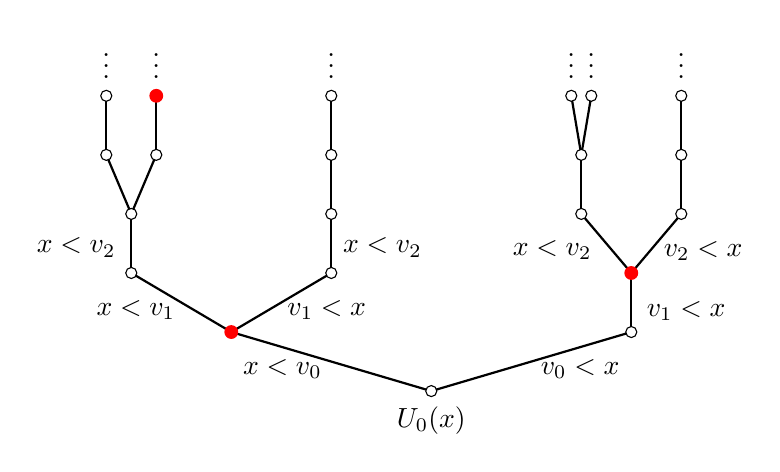
\begin{tikzpicture}[grow'=up,scale=.5]
\tikzstyle{level 1}=[sibling distance=4in]
\tikzstyle{level 2}=[sibling distance=2in]
\tikzstyle{level 3}=[sibling distance=1in]
\tikzstyle{level 4}=[sibling distance=0.5in]
\tikzstyle{level 5}=[sibling distance=0.2in]
\tikzstyle{level 6}=[sibling distance=0.1in]
\tikzstyle{level 7}=[sibling distance=0.07in]

\node {} coordinate (t9)
child{ coordinate (t0) edge from parent[color=black,thick]
child{coordinate (t00) edge from parent[color=black,thick]
child{coordinate (t000) edge from parent[color=black,thick]
child{coordinate (t0000) edge from parent[color=black,thick]
child{coordinate (t00000) edge from parent[color=black,thick]}
}%endparen for t0000
child{coordinate (t0001) edge from parent[color=black,thick]
child{coordinate (t00010) edge from parent[color=black,thick]}
}%endparen for t0001
}%endparen for t000
}%endparen for t00
child{coordinate (t01) edge from parent[color=black,thick]
child{coordinate (t010) edge from parent[color=black,thick]
child{coordinate (t0100) edge from parent[color=black,thick]
child{coordinate (t01000) edge from parent[color=black,thick]}
}%endparen for t0100
}%endparen for t010
}%endparen for t01
}%endparen for t0
child{ coordinate (t1) edge from parent[color=black,thick]
child{coordinate (t10) edge from parent[color=black,thick]
child{coordinate (t100) edge from parent[color=black,thick]
child{coordinate (t1000) edge from parent[color=black,thick]
child{coordinate (t10000) edge from parent[color=black,thick]}
child{coordinate (t10001) edge from parent[color=black,thick]}
}%endparen for t1000
}%endparen for t100
child{coordinate (t101) edge from parent[color=black,thick]
child{coordinate (t1010) edge from parent[color=black,thick]
child{coordinate (t10100) edge from parent[color=black,thick]}
}%endparen for t1010
}%endparen for t101
}%endparen for t10
};%endparen for t1
%
%colored nodes in left tree
\node[label=20:\hspace*{5mm}$v_1<x$,label=160:$x<v_1$\hspace*{5mm},circle, fill=red,inner sep=0pt, minimum size=5pt] at (t0) {};
\node[label=150:$x<v_2\hspace{3mm}$,label=20:$\hspace{2mm}v_2<x$,circle, fill=red,inner sep=0pt, minimum size=5pt] at (t10) {};
\node[circle, fill=red,inner sep=0pt, minimum size=5pt] at (t00010) {};

%dots going up
\node[circle,inner sep=0pt, minimum size=5pt,label=90:$\vdots$] at (t00000) {};
\node[circle,inner sep=0pt, minimum size=5pt,label=90:$\vdots$] at (t00010) {};
\node[circle,inner sep=0pt, minimum size=5pt,label=90:$\vdots$] at (t01000) {};
\node[circle,inner sep=0pt, minimum size=5pt,label=90:$\vdots$] at (t10000) {};
\node[circle,inner sep=0pt, minimum size=5pt,label=90:$\vdots$] at (t10001) {};
\node[circle,inner sep=0pt, minimum size=5pt,label=90:$\vdots$] at (t10100) {};

%empty bubble nodes
\node[label=150:$x<v_0\hspace{12mm}$,label=270:$U_0(x)$,label=30:$\hspace{12mm}v_0<x$,circle, fill=white,draw,inner sep=0pt, minimum size=4pt] at (t9) {};
\node[label=90:$x<v_2\hspace{14mm}$,circle, fill=white,draw,inner sep=0pt, minimum size=4pt] at (t00) {};
\node[circle, fill=white,draw,inner sep=0pt, minimum size=4pt] at (t000) {};
\node[circle, fill=white,draw,inner sep=0pt, minimum size=4pt] at (t0000) {};
\node[circle, fill=white,draw,inner sep=0pt, minimum size=4pt] at (t00000) {};
\node[circle, fill=white,draw,inner sep=0pt, minimum size=4pt] at (t0001) {};
\node[label=90:$\hspace{13mm}x<v_2$,circle, fill=white,draw,inner sep=0pt, minimum size=4pt] at (t01) {};
\node[circle, fill=white,draw,inner sep=0pt, minimum size=4pt] at (t010) {};
\node[circle, fill=white,draw,inner sep=0pt, minimum size=4pt] at (t0100) {};
\node[circle, fill=white,draw,inner sep=0pt, minimum size=4pt] at (t01000) {};
\node[label=20:$v_1<x$,circle, fill=white,draw,inner sep=0pt, minimum size=4pt] at (t1) {};
\node[circle, fill=white,draw,inner sep=0pt, minimum size=4pt] at (t100) {};
\node[circle, fill=white,draw,inner sep=0pt, minimum size=4pt] at (t1000) {};
\node[circle, fill=white,draw,inner sep=0pt, minimum size=4pt] at (t10000) {};
\node[circle, fill=white,draw,inner sep=0pt, minimum size=4pt] at (t10001) {};
\node[circle, fill=white,draw,inner sep=0pt, minimum size=4pt] at (t101) {};
\node[circle, fill=white,draw,inner sep=0pt, minimum size=4pt] at (t1010) {};
\node[circle, fill=white,draw,inner sep=0pt, minimum size=4pt] at (t10100) {};
\end{tikzpicture}
\end{minipage}
\begin{minipage}{.2\textwidth}
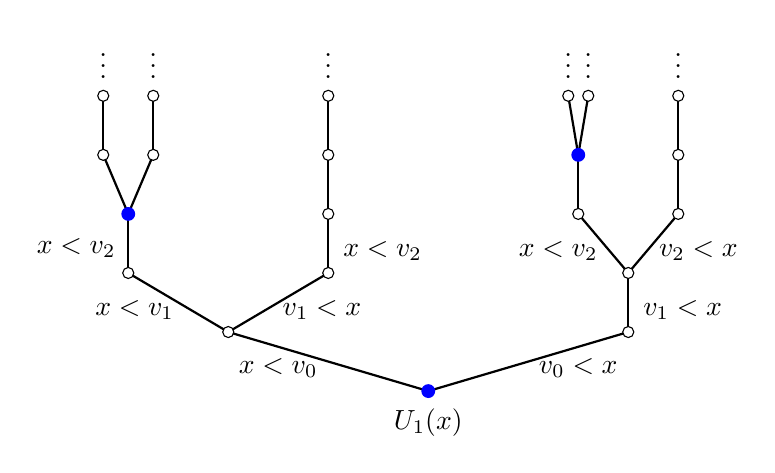
\begin{tikzpicture}[grow'=up,scale=.5]
\tikzstyle{level 1}=[sibling distance=4in]
\tikzstyle{level 2}=[sibling distance=2in]
\tikzstyle{level 3}=[sibling distance=1in]
\tikzstyle{level 4}=[sibling distance=0.5in]
\tikzstyle{level 5}=[sibling distance=0.2in]
\tikzstyle{level 6}=[sibling distance=0.1in]
\tikzstyle{level 7}=[sibling distance=0.07in]

\node {} coordinate (u9)
child{coordinate (u0) edge from parent[color=black,thick]
child{coordinate (u00) edge from parent[color=black,thick]
child{coordinate (u000) edge from parent[color=black,thick]
child{coordinate (u0000) edge from parent[color=black,thick]
child{coordinate (u00000) edge from parent[color=black,thick]}
}%endparen for u0000
child{coordinate (u0001) edge from parent[color=black,thick]
child{coordinate (u00010) edge from parent[color=black,thick]}
}%endparen for u0001
}%endparen for u000
}%endparen for u00
child{coordinate (u01) edge from parent[color=black,thick]
child{coordinate (u010) edge from parent[color=black,thick]
child{coordinate (u0100) edge from parent[color=black,thick]
child{coordinate (u01000) edge from parent[color=black,thick]}
}%endparen for u0100
}%endparen for u010
}%endparen for u01
}%endparen for u0
child{coordinate (u1) edge from parent[color=black,thick]
child{coordinate (u10) edge from parent[color=black,thick]
child{coordinate (u100) edge from parent[color=black,thick]
child{coordinate (u1000) edge from parent[color=black,thick]
child{coordinate (u10000) edge from parent[color=black,thick]}%endparen for u10000
child{coordinate (u10001) edge from parent[color=black,thick]}
}%endparen for u1000
}%endparen for u100
child{coordinate (u101) edge from parent[color=black,thick]
child{coordinate (u1010) edge from parent[color=black,thick]
child{coordinate (u10100) edge from parent[color=black,thick]}
}%endparen for u1010
}%endparen for u101
}%endparen for u10
};%endparen for u1

%blue nodes for the right tree
\node[label=150:$x<v_0\hspace{12mm}$,label=30:$\hspace{12mm}v_0<x$,label=270:$U_1(x)$,circle, fill=blue,inner sep=0pt, minimum size=5pt] at (u9) {};
\node[circle, fill=blue,inner sep=0pt, minimum size=5pt] at (u000) {};
\node[circle, fill=blue,inner sep=0pt, minimum size=5pt] at (u1000) {};

%dots going up for the right tree
\node[circle,inner sep=0pt, minimum size=5pt,label=90:$\vdots$] at (u00000) {};
\node[circle,inner sep=0pt, minimum size=5pt,label=90:$\vdots$] at (u00010) {};
\node[circle,inner sep=0pt, minimum size=5pt,label=90:$\vdots$] at (u01000) {};
\node[circle,inner sep=0pt, minimum size=5pt,label=90:$\vdots$] at (u10000) {};
\node[circle,inner sep=0pt, minimum size=5pt,label=90:$\vdots$] at (u10001) {};
\node[circle,inner sep=0pt, minimum size=5pt,label=90:$\vdots$] at (u10100) {};

%empty circle nodes
\node[label=150:$x<v_1\hspace{5mm}$,label=30:$\hspace{5mm}v_1<x$,circle, fill=white,draw,inner sep=0pt, minimum size=4pt] at (u0) {};
\node[label=120:$x<v_2$,circle, fill=white,draw,inner sep=0pt, minimum size=4pt] at (u00) {};
\node[circle, fill=white,draw,inner sep=0pt, minimum size=4pt] at (u0000) {};
\node[circle, fill=white,draw,inner sep=0pt, minimum size=4pt] at (u00000) {};
\node[circle, fill=white,draw,inner sep=0pt, minimum size=4pt] at (u0001) {};
\node[circle, fill=white,draw,inner sep=0pt, minimum size=4pt] at (u00010) {};
\node[label=30:$x<v_2$,circle, fill=white,draw,inner sep=0pt, minimum size=4pt] at (u01) {};
\node[circle, fill=white,draw,inner sep=0pt, minimum size=4pt] at (u010) {};
\node[circle, fill=white,draw,inner sep=0pt, minimum size=4pt] at (u0100) {};
\node[circle, fill=white,draw,inner sep=0pt, minimum size=4pt] at (u01000) {};
\node[label=30:$v_1<x$,circle, fill=white,draw,inner sep=0pt, minimum size=4pt] at (u1) {};
\node[label=150:$x<v_2\hspace{2mm}$,label=30:$\hspace{2mm}v_2<x$,circle, fill=white,draw,inner sep=0pt, minimum size=4pt] at (u10) {};
\node[circle, fill=white,draw,inner sep=0pt, minimum size=4pt] at (u100) {};
\node[circle, fill=white,draw,inner sep=0pt, minimum size=4pt] at (u10000) {};
\node[circle, fill=white,draw,inner sep=0pt, minimum size=4pt] at (u10001) {};
\node[circle, fill=white,draw,inner sep=0pt, minimum size=4pt] at (u101) {};
\node[circle, fill=white,draw,inner sep=0pt, minimum size=4pt] at (u1010) {};
\node[circle, fill=white,draw,inner sep=0pt, minimum size=4pt] at (u10100) {};
\end{tikzpicture}
\end{minipage}

\end{center}
\begin{tikzpicture}
%the nodes along the bottom
\node[circle, fill=blue,inner sep=0pt, minimum size=5pt, label=$v_3$] (v3) {};
\node[circle, fill=red,inner sep=0pt, minimum size=5pt,label=$v_5$,right=2cm of v3] (v5) {};
\node[circle, fill=red,inner sep=0pt, minimum size=5pt,label=$v_1$,right=2cm of v5] (v1) {};
\node[circle, fill=blue,inner sep=0pt, minimum size=5pt, label=$v_0$,right=2cm of v1] (v0) {};
\node[circle, fill=blue,inner sep=0pt, minimum size=5pt,label=$v_4$,right=2cm of v0] (v4) {};
\node[circle, fill=red,inner sep=0pt, minimum size=5pt,label=$v_2$,right=2cm of v4] (v2) {};
\end{tikzpicture}
\end{document}

%Still need:
%node labels
%edge labels